\documentclass[17pt]{beamer}
\usepackage[utf8]{inputenc}
\usepackage[T1]{fontenc}
\usepackage{listings}
\usepackage{themes/dbt}
\usepackage{textpos}
\usepackage{xcolor,pgf}
\lstset{language=csh, numbers=left, frame=single, breaklines=true, breakatwhitespace=false, basicstyle=\smaller, numberstyle=\small, basicstyle=\sffamily}

%\usetheme{Warsaw}
\title{The road to containerization}
\institute{
\includegraphics[width=4cm]{images/title_logo.png}}
\author{Wiesław Kielas}
\date{\today}

\defbeamertemplate*{title page}{customized}[1][]
{
  \usebeamercolor[fg]{title}
  \usebeamerfont{title}\inserttitle\par
  \bigskip
  \bigskip
  \usebeamerfont{institute}\insertinstitute\par
  \bigskip
  \bigskip
  \usebeamercolor[fg]{item}
  \usebeamerfont{author}\insertauthor\par
  \usebeamerfont{date}October 4, 2018\par
}

\newcommand{\imageframe}[2]{{
  \usebackgroundtemplate{\includegraphics[width=\paperwidth,height=\paperheight]
  {#1}}
  \begin{frame}{
    \vspace{-6pt}\usebeamercolor[fg]{item}
    \pgfsetfillopacity{0.8}
    \begin{snugshade}
    \centering #2
    \end{snugshade}
  }
  \end{frame}
}}

\begin{document}
  \begin{frame}
    \maketitle
  \end{frame}

  \logo{\vspace{-6pt}
\includegraphics[width=1.0cm]{images/logo.png}}

  \begin{frame}{What is this about?}
  \begin{itemize}
    \item<1-> About me
    \begin{itemize}
      \item Started at GAT two years ago
      \item IT professional since 2011
      \item Only DevOps engineer
      \item First time event speaker
    \end{itemize}
    \bigskip
    \item<2-> What will I~talk about?
    \begin{itemize}
      \item Why throw the Chef stack away?
      \item How containers helped?
      \item What did we learn?
    \end{itemize}
  \end{itemize}
  \end{frame}

  % ---------------------------------- %

  \imageframe{images/ancient_history.jpg}{Ancient history}

  \begin{frame}{The year is 2016}
  \centering
  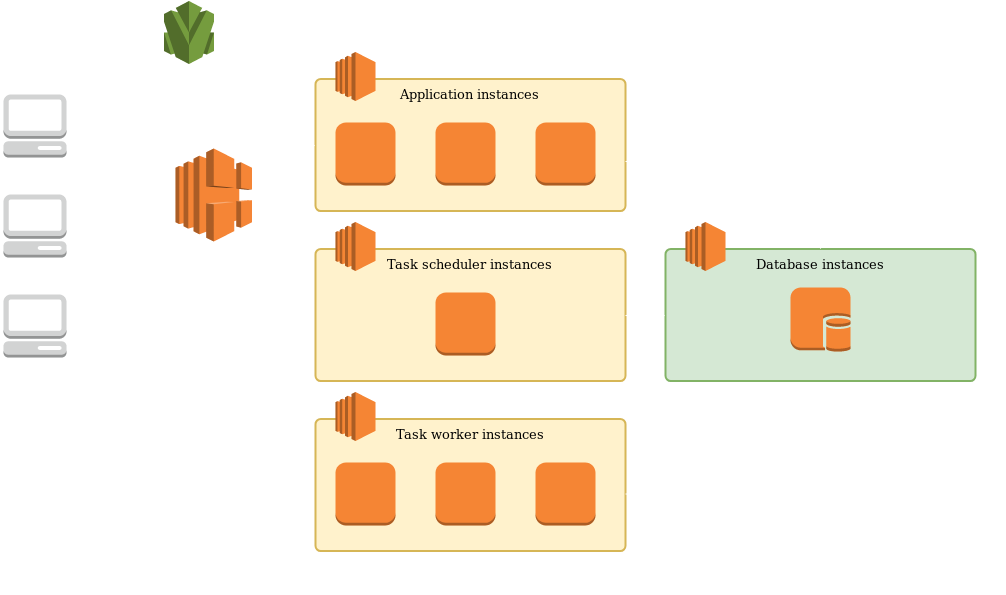
\includegraphics[width=11cm]{images/opsworks_diagram.png}
  \end{frame}

  \begin{frame}{Pain points explained}
  \begin{itemize}
    \item<1-> Long deployment times
    \item<2-> Uncertainty of success
    \item<3-> Deployments caused downtime
    \item<4-> Wasting resources = high cost
    \item<5-> Not automated
  \end{itemize}
  \end{frame}

  \begin{frame}{What next?}
  \begin{itemize}
    \item<1-> Improve existing infrastructure
    \begin{itemize}
      \item Vendor lock-in
      \item Hard to lower costs
    \end{itemize}
    \bigskip
    \item<2-> Move to containers
    \begin{itemize}
      \item Save money
      \item Lessen configuration complexity
      \item Play with shiny new tools
    \end{itemize}
  \end{itemize}
  \end{frame}

  % ---------------------------------- %

  \imageframe{images/container_landscape.jpg}{The container landscape}

  \begin{frame}{Docker}
    \begin{columns}[c]
      \begin{column}{.2\textwidth}
          
\includegraphics[width=3cm,height=3cm]{images/docker_logo.png}
      \end{column}
      \begin{column}{.8\textwidth}
        \begin{itemize}
          \item Container platform
          \item Lightweight VMs
          \item Packaging format
          \begin{itemize}
            \item Reproducible deployments
          \end{itemize}
        \end{itemize}
      \end{column}
    \end{columns}
  \end{frame}

  \begin{frame}{Kubernetes}
    \begin{columns}[c]
      \begin{column}{.2\textwidth}
          
\includegraphics[width=3cm,height=3cm]{images/kubernetes_logo.png}
      \end{column}
      \begin{column}{.8\textwidth}
        \begin{itemize}
          \item Container orchestration
          \item Service discovery
          \item Persistent storage
          \item High availability
        \end{itemize}
      \end{column}
    \end{columns}
  \end{frame}

  \begin{frame}{Helm}
    \begin{columns}[c]
      \begin{column}{.2\textwidth}
          
\includegraphics[width=3cm,height=3cm]{images/helm_logo.png}
      \end{column}
      \begin{column}{.8\textwidth}
        \begin{itemize}
          \item Package manager
          \item Provides templates
          \begin{itemize}
            \item Configuration management
          \end{itemize}
          \item Deployment management
        \end{itemize}
      \end{column}
    \end{columns}
  \end{frame}

  % ---------------------------------- %

  \imageframe{images/migrating_cranes.jpg}{Migrating to Kubernetes}

  \begin{frame}{Why move to GKE?}
  \begin{itemize}
    \item<1-> Kubernetes as a~Service
    \item<2-> Automates the management plane
    \item<3-> Automated the scary cluster deployment
    \item<4-> Built in goodies:
    \begin{itemize}
      \item Integrated authentication
      \item Centralized logging
      \item Cluster monitoring
      \item Container registry
    \end{itemize}
  \end{itemize}
  \end{frame}

  \begin{frame}{The journey}
  \begin{itemize}
    \item<1-> Docker images for applications
    \item<2-> CI pipeline modification
    \item<3-> Helm instead of Chef
    \begin{itemize}
      \item Change configuration generation
    \end{itemize}
    \bigskip
    \item<4-> Moving apps one by one
  \end{itemize}
  \end{frame}

  \begin{frame}{The end result}
  \centering
  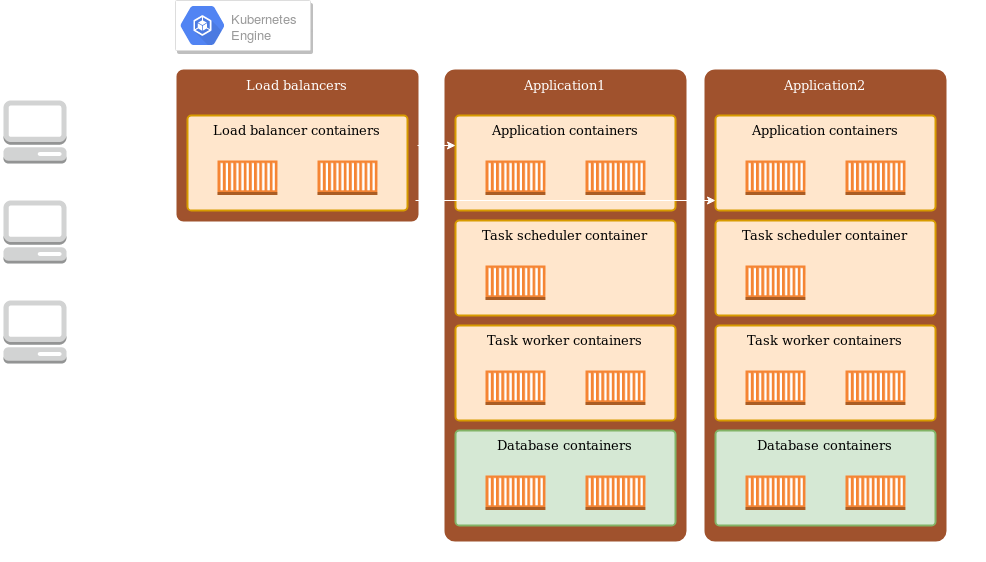
\includegraphics[width=11cm]{images/kubernetes_diagram.png}
  \end{frame}

  \begin{frame}{Pain points revisited}
  \begin{itemize}
    \item<1-> Long deployment times
    \begin{itemize}
      \item Down from 15 minutes to 1-2 minutes
    \end{itemize}
    \item<2-> Uncertainty of success
    \begin{itemize}
      \item Deployments were predictable
    \end{itemize}
    \item<3-> Deployments caused downtime
    \begin{itemize}
      \item Rolling deployments = no downtime
    \end{itemize}
    \item<4-> High cost
    \begin{itemize}
      \item Lowered
    \end{itemize}
    \item<5-> Not automated
    \begin{itemize}
      \item Automated (after some time)
    \end{itemize}
  \end{itemize}
  \end{frame}

  \imageframe{images/dumpster_fire.jpg}{Whoops!}

  \begin{frame}{No happy end}
  \begin{itemize}
    \item<1-> Bugs!
    \begin{itemize}
      \item Nodes crashing
      \item Networking problems
    \end{itemize}
    \item<2-> Bad support
    \item<3-> Kubernetes as a~Service
    \begin{itemize}
      \item Frustrating when it doesn't work
    \end{itemize}
    \item<4-> Inflexible configuration
    \begin{itemize}
      \item Caching images possible with own CM
    \end{itemize}
    \item<5-> Waiting for security updates
  \end{itemize}
  \end{frame}

  \imageframe{images/returning_cranes.jpg}{Migrating back to AWS}

  \begin{frame}{Enter kops}
  \begin{columns}[c]
    \begin{column}{.3\textwidth}
      
\includegraphics[width=4cm]{images/kops_logo.png}
    \end{column}
    \begin{column}{.7\textwidth}
      \begin{itemize}
        \item Cluster bootstrapping utility
        \item Lifecycle management
        \item Very flexible
        \begin{itemize}
          \item Custom IAM roles
          \item Caching images
          \item Changing daemon configuration
        \end{itemize}
      \end{itemize}
    \end{column}
  \end{columns}
  \end{frame}

  \begin{frame}{New challenges}
  \begin{itemize}
    \item<1-> Missing parts
    \begin{itemize}
      \item Integrated authentication - \textbf{PKI}
      \item Centralized logging - \textbf{Graylog}
      \item Cluster monitoring - \textbf{Prometheus}
    \end{itemize}
    \item<2-> Moving stuff
    \begin{itemize}
      \item Rewriting helper scripts
      \item Load balancers behave differently
      \item Use EBS instead of Google disks
      \item Container registry - \textbf{Amazon ECR}
    \end{itemize}
  \end{itemize}
  \end{frame}

  \imageframe{images/feels_good_man.jpg}{The end result}

  \begin{frame}{Lessons learned}
  \begin{itemize}
    \item<1-> Outsourcing service management gives a~big head start
    \item<2-> Support is extremely important
    \item<3-> Cloud agnostic design can return very quickly
  \end{itemize}
  \end{frame}

  \imageframe{images/questions.jpg}{Questions?}

\end{document}
